%Este trabalho está licenciado sob a Licença Atribuição-CompartilhaIgual 4.0 Internacional Creative Commons. Para visualizar uma cópia desta licença, visite http://creativecommons.org/licenses/by-sa/4.0/deed.pt_BR ou mande uma carta para Creative Commons, PO Box 1866, Mountain View, CA 94042, USA.

\chapter{Problema de Valor de Contorno}\label{cap_pvc}
\thispagestyle{fancy}

Neste capítulo, \hl{estudamos métodos numéricos para resolver \emph{Problemas de Valores de Contorno}} da forma
\begin{subequations}\hleq
  \begin{align}
    &u'' = f(x, u, u'), ~a < x < b,\\
    &\eta_1 u'(a) + \theta_1 u(b) = g_1\\
    &\eta_2 u'(b) + \theta_2 u(b) = g_2
\end{align}
\end{subequations}
onde a incógnita é $u = u(x)$ com dada $f = f(x, u, u')$ e dados parâmetros $\eta_1$, $\theta_1$ (não simultaneamente nulos), $\eta_2$, $\theta_2$ (não simultaneamente nulos), $g1$ e $g2$.

\section{Método de Diferenças Finitas}\label{cap_pvc_sec_mdf}

Consideramos o seguinte problema linear de valor de contorno (PVC)
\begin{subequations}\label{cap_pvc_sec_mdf:eq:pvc}\hleq
  \begin{align}
    &u'' + \alpha(x) u' + \beta(x) u = f(x), ~a < x < b, \label{cap_pvc_sec_mdf:eq:pvc_eq}\\
    &u(a) = g, \label{cap_pvc_sec_mdf:eq:pvc_bc1}\\
    &u(b) = h. \label{cap_pvc_sec_mdf:eq:pvc_bc2}
  \end{align}
\end{subequations}
onde a incógnita é $u = u(x)$ com dada fonte $f = f(x)$ e dados parâmetros $g$ e $h$.

\hl{A aproximação pelo \emph{Método de Diferenças Finitas} (MDF) de {\eqref{cap_pvc_sec_mdf:eq:pvc_eq}}-{\eqref{cap_pvc_sec_mdf:eq:pvc_bc2}} surge da substituição das derivadas por Fórmulas de Diferenças Finitas}. De forma geral, o método pode ser dividido em três etapas: 1. discretização do domínio, 2. discretização das equações, 3. resolução do problema discreto.

\begin{flushleft}
  \emph{1. Discretização do Domínio}
\end{flushleft}

\hl{A \emph{discretização do domínio} é seu particionamento em \emph{subintervalos} (\emph{células} computacionais) e \emph{pontos} (\emph{nodos} computacionais)}. Por simplicidade, vamos considerar apenas o caso de um particionamento uniforme. Particionamos o domínio $D = [a, b]$ em $n$ de subintervalos de \emph{tamanho de malha}
\begin{equation}\hleq
  h = \frac{b-a}{n},
\end{equation}
e os nodos da partição podem ser indexados da seguinte forma
\begin{equation}\hleq
  x_i = a + (i-1)h,
\end{equation}
com $i = 1, 2, 3, \dotsc, n+1$.

\begin{flushleft}
  {\bf 2. Discretização das Equações}
\end{flushleft}

Começando por \eqref{cap_pvc_sec_mdf:eq:pvc_eq}, em um nodo \hl{$x=x_i$, $i=2, 3, \dotsc, n$}, temos
\begin{equation}\label{cap_pvc_sec_mdf:eq:pvc_eq_no_ponto}
  u''(x_i) + \alpha(x_i) u'(x_i) + \beta(x_i) u(x_i) = f(x_i).
\end{equation}
Podemos substituir a segunda derivada de $u$ pela \emph{fórmula de diferenças finitas} central de ordem $h^2$
\begin{equation}
  u''(x_i) = \underbrace{\frac{u(x_i-h) - 2u(x_i) + u(x_i+h)}{h^2}}_{D^2_{0,h^2}u(x_i)} + O(h^2).
\end{equation}
A primeira derivada de $u$ também pode ser substituída pela fórmula de diferenças finitas central de ordem $h^2$
\begin{equation}
  u'(x_i) = \underbrace{\frac{u(x_i+h)-u(x_i-h)}{2h}}_{D_{0,h^2}u(x_i)} + O(h^2).
\end{equation}

Agora, denotando \hl{$u_i \approx u(x_i)$}, temos $u_{i-1}\approx u(x_i-h)$ e $u_{i+1}\approx u(x_i+h)$. Substituindo as derivadas pelas fórmulas de diferenças finitas, temos de \eqref{cap_pvc_sec_mdf:eq:pvc_eq_no_ponto} que
\begin{equation}
  \begin{aligned}
    &\left(\frac{u_{i-1}-2u_i+u_{i+1}}{h^2}\right) + \alpha(x_i)\left(\frac{u_{i+1}-u_{i-1}}{2h}\right) \\
    &\quad + \beta(x_i)u_i + O(h^2) = f(x_i),
  \end{aligned}
\end{equation}
Rearranjando os termos e desconsiderando o termo do erro de truncamento, obtemos o seguinte sistema de equações lineares
\begin{equation}\label{cap_pvc_sec_mdf:eq:pvc_mdf_sis1}
  \begin{aligned}
    &\left(\frac{1}{h^2}-\frac{\alpha_i}{2h}\right)u_{i-1} + \left(\beta_i - \frac{2}{h^2}\right)u_i\\
    &\quad + \left(\frac{1}{h^2}+\frac{\alpha_i}{2h}\right)u_{i+1} = f_i, 
  \end{aligned}
\end{equation}
onde, usamos a notação $\alpha_i = \alpha(x_i)$, $\beta_i = \beta(x_i)$ e $f_i = f(x_i)$.

Observamos que este sistema consiste em $n-1$ equações envolvendo as $n+1$ incógnitas $u_i$, $i=1, 2, \dotsc, n+1$. Para fechá-lo, usamos as condições de contorno. De \eqref{cap_pvc_sec_mdf:eq:pvc_bc1}, temos
\begin{equation}\label{cap_pvc_sec_mdf:eq:pvc_mdf_sis0}
  u_1 = g
\end{equation}
e de \eqref{cap_pvc_sec_mdf:eq:pvc_bc2} temos
\begin{equation}\label{cap_pvc_sec_mdf:eq:pvc_mdf_sis2}
  u_{n+1} = h,
\end{equation}
lembrando que $u_0\approx u(x_0)$ e $u_n\approx u(x_n)$.

Por fim, as equações \eqref{cap_pvc_sec_mdf:eq:pvc_mdf_sis1}-\eqref{cap_pvc_sec_mdf:eq:pvc_mdf_sis2} formam o seguinte \emph{problema discretizado}
\begin{subequations}\label{cap_pvc_sec_mdf:eq:pd}\hleq
  \begin{align}
    &u_1 = g,\\
    &~\nonumber\\
    &\left(\frac{1}{h^2}-\frac{\alpha_i}{2h}\right)u_{i-1} + \left(\beta_i - \frac{2}{h^2}\right)u_i \nonumber\\
    &\quad + \left(\frac{1}{h^2}+\frac{\alpha_i}{2h}\right)u_{i+1} = f_i,\\
    &~\nonumber\\
    &u_{n+1} = h,
  \end{align}
\end{subequations}
para $i = 2, 3, \dotsc, n$.

\begin{flushleft}
  {\bf 3. Resolução do problema discreto}
\end{flushleft}

\hl{O problema discreto {\eqref{cap_pvc_sec_mdf:eq:pd}} consiste em um sistema linear de $n+1$ equações com $n+1$ incógnitas}. Na forma matricial temos
\begin{equation}\eqref{cap_pvc_sec_mdf:eq:sis_mdf}
  A\pmb{u} = \pmb{b}
\end{equation}
onde $\pmb{u} = (u_1, u_2, \dotsc, u_{n+1})$ é o vetor das incógnitas, $\pmb{b} = (g, f_2, f_3, \dotsc, f_{n}, h)$. A matriz dos coeficientes é  $A = [a_{i,j}]_{i,j=1}^{n+1,n+1}$ e seus elementos não nulos são
\begin{align}
  &a_{1,1} = 1,
  & ~ \nonumber \\
  &a_{i,i-1} = \frac{1}{h^2}-\frac{\alpha_i}{2h},\\
  &a_{i,i} = \beta_i - \frac{2}{h^2}, \\
  &a_{i,i+1} = \frac{1}{h^2}+\frac{\alpha_i}{2h},\\
  & ~ \nonumber \\
  &a_{n+1,n+1} = 1,
\end{align}
para $i = 2, 3, \dotsc, n$.

\hl{A resolução do sistema discreto se resume, a resolver o sistema $A\pmb{u} = \pmb{b}$}, o que pode ser feito por qualquer método numérico apropriado.

\begin{ex}\label{cap_pvc_sec_mdf:ex:pvc_mdf_1}
  Consideramos o seguinte PVC
  \begin{align}
    &-u'' = \pi^2\sen(\pi x), ~0 < x < 1,\\
    &u(0) = 0,\\
    &u(1) = 0.
  \end{align}

\begin{figure}[h!]
  \centering
  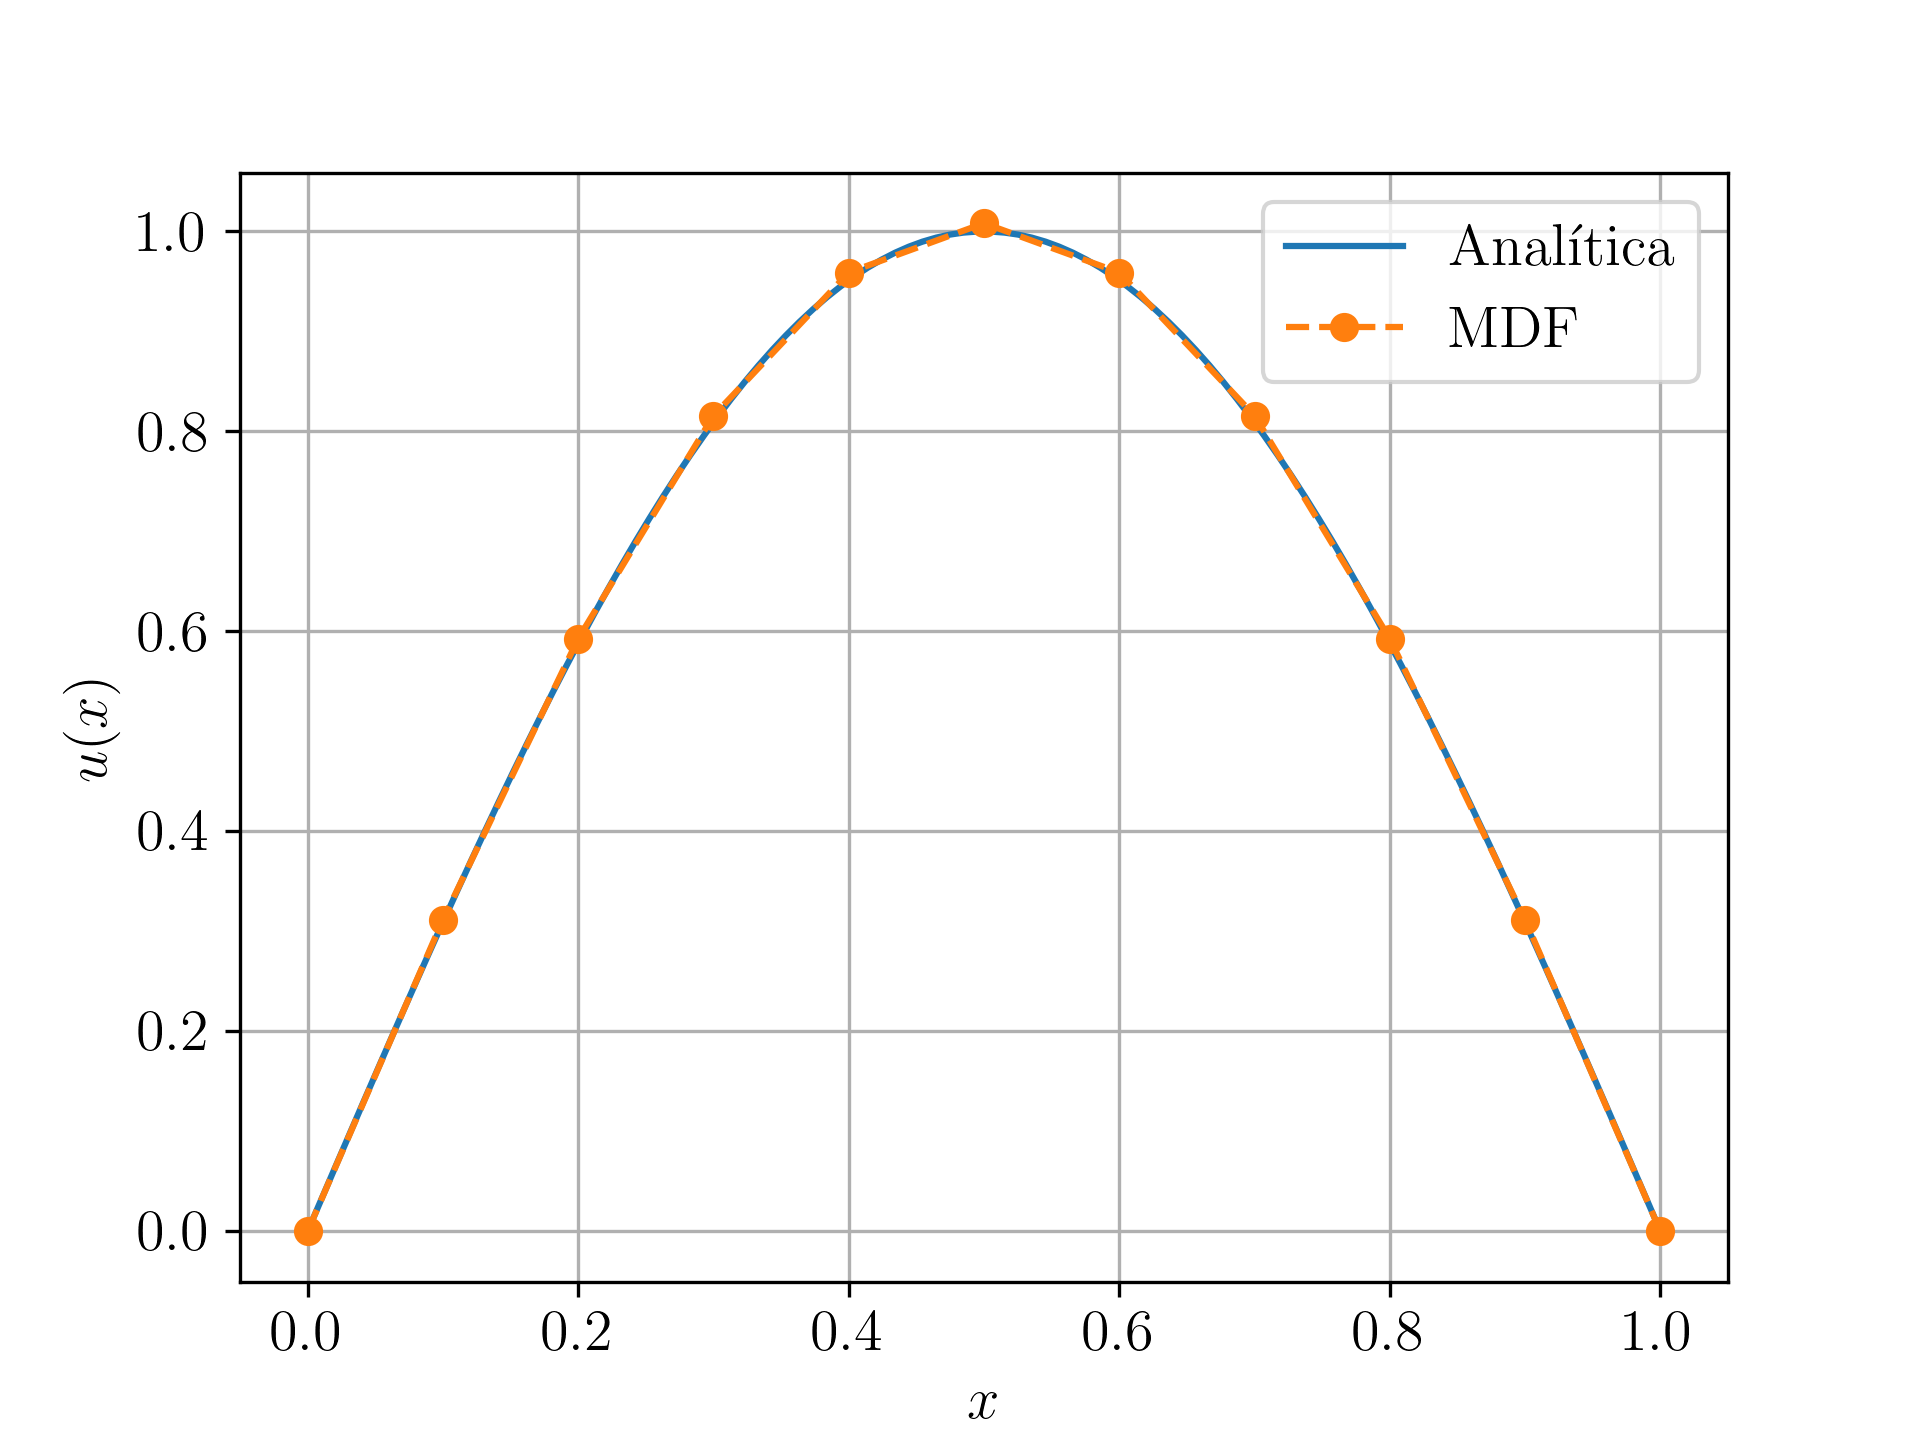
\includegraphics[width=0.8\textwidth]{./cap_pvc/dados/fig_mdf/fig}
  \caption{Resultado referente ao Exemplo~\ref{cap_pvc_sec_mdf:ex:pvc_mdf_1}.}
  \label{cap_pvc_sec_mdf:fig:ex_pvc_mdf_1}
\end{figure}

A solução analítica deste problema é $u(x) = \sen(\pi x)$. Usando o MDF como acima, encontramos o problema discreto
\begin{subequations}
  \begin{align}
    u_1 &= 0,\\
    -\frac{1}{h^2}u_{i-1} + \frac{2}{h^2}u_i - \frac{1}{h^2}u_{i+1} &= \pi^2\sen(\pi x_i),\\
    u_{n+1} &= 0,
  \end{align}
\end{subequations}
com tamanho de malha $h=1/n$ e nodos $x_i = (i-1)h$ indexados por $i = 1, 2, \dotsc, n+1$.

\begin{table}[h!]
  \centering
  \caption{Resultados referentes ao Exemplo~\ref{cap_pvc_sec_mdf:ex:pvc_mdf_1}.}
  \begin{tabular}{l|c}\toprule
    $h$ & $\|\tilde{u} - u\|_{L^2}$ \\\midrule
    $1.0\e-1$ & $1.8\e-2$\\
    $5.0\e-2$ & $6.5\e-3$\\
    $2.5\e-2$ & $2.3\e-3$\\
    $1.0\e-3$ & $5.8\e-4$\\\bottomrule
  \end{tabular}
  \label{cap_pvc_sec_mdf:tab:ex_pvc_mdf_1}
\end{table}

Resolvendo este sistema com $h=10^{-1}$ obtemos a solução numérica apresentada na Figura~\ref{cap_pvc_sec_mdf:fig:ex_pvc_mdf_1}. Ainda, na Tabela~\ref{cap_pvc_sec_mdf:tab:ex_pvc_mdf_1} temos a comparação na norma $L^2$ da solução numérica $\tilde{\pmb{u}}$ com a solução analítica $\pmb{u} = (u(x_i))_{i=1}^{n+1}$ para diferentes escolhas de $h$.

\begin{lstlisting}[caption=pvc\_mdf.py]
import numpy as np

# malha
n = 10
h = 1./n
xx = np.linspace(0., 1., n+1)

# fonte
def f(x):
    return np.pi**2*np.sin(np.pi*x)

# prob discreto
A = np.zeros((n+1, n+1))
b = np.empty(n+1)

# c.c. x = 0.
A[0,0] = 1.
b[0] = 0.

# pts internos
for i in range(1,n):
    A[i,i-1] = -1./h**2
    A[i,i] = 2./h**2
    A[i,i+1] = -1./h**2
    b[i] = f(xx[i])

# c.c. x = 1.
A[n,n] = 1.
b[n] = 0.

# resol
u = npla.solve(A, b)
\end{lstlisting}
\end{ex}

\subsection{Exercícios}

\begin{exer}
  Considere o PVC
  \begin{align}
    &-u'' = \pi^2\cos(\pi x), ~0 < x < 1,\\
    &u(0) = 1,\\
    &u(1) = -1.
  \end{align}
  A solução analítica deste problema é $u(x) = \cos(\pi x)$. Use o MDF para computar aproximações numéricas $\tilde{\pmb{u}}_h$ com tamanhos de malha $h=10^{-1}, 10^{-2}, 10^{-3}, 10^{-4}$ e verifique o erro absoluto $\varepsilon_{\text{abs}} := \|\tilde{\pmb{u}}_h - \pmb{u}\|$.
\end{exer}
\begin{resp}
  \begin{tabular}{l|c}\toprule
    $h$ & $\|\tilde{u} - u\|_{L^2}$ \\\midrule
    $10^{-1}$ & $3.9\e-3$\\
    $10^{-2}$ & $1.2\e-4$\\
    $10^{-3}$ & $3.9\e-6$\\
    $10^{-4}$ & $1.2\e-7$\\\bottomrule
  \end{tabular}  
\end{resp}

\begin{exer}
  Considere o PVC
  \begin{align}
    &-u'' = 1, ~-1 < x < 1,\\
    &u(-1) = 0,\\
    &u(1) = 0.
  \end{align}
  A solução analítica deste problema é $u(x) = 1-x^2$. Use o MDF com $n=20$ subintervalos na malha e verifique o erro absoluto $\varepsilon_{\text{abs}} := \|\tilde{\pmb{u}}_h - \pmb{u}\|$. Por que o erro está próximo precisão de máquina? Justifique sua resposta.
\end{exer}
\begin{resp}
  $\varepsilon_{\text{abs}} = 3.1\e-14$.
\end{resp}

\begin{exer}
Considere o seguinte PVC
\begin{subequations}
  \begin{align}
    &-u'' + u' = f(x), ~-1 < x < 1,\\
    &u(-1) = 0,\\
    &u'(1) =0,
  \end{align}
\end{subequations}
onde
\begin{equation}
  f(x) = \left\{
    \begin{array}{ll}
      1 &, x\leq 0\\
      0 &, x>0
    \end{array}
  \right.
\end{equation}
Use uma aproximação adequada pelo método de diferenças finitas para obter o valor aproximado de $u(0)$ com precisão de $2$ dígitos significativos.
\end{exer}
\begin{resp}
  $7,2\E-1$
\end{resp}

\begin{exer}
  Considere o PVC
  \begin{align}
    &-u'' = \pi^2\cos(\pi x), ~0 < x < 1,\\
    &u(0) = 1,\\
    &u'(1) = 0.
  \end{align}
  A solução analítica deste problema é $u(x) = \cos(\pi x)$. Aplique o MDF para computar aproximações numéricas usando a:
  \begin{enumerate}[a)]
  \item fórmula de diferenças finitas $D_{-,h}u(x)$ no contorno $x=1$.
  \item fórmula de diferenças finitas $D_{-,h^2}u(x)$ no contorno $x=1$.
  \end{enumerate}
  Quais das duas produz o resultado mais preciso? Justifique sua resposta.
\end{exer}
\begin{resp}
  b) resultado mais preciso.
\end{resp}

\section{Método de Elementos Finitos}\label{cap_pvc_sec_fem}

Consideramos o seguinte problema linear de valor de contorno (PVC)
\begin{subequations}\label{cap_pvc_sec_fem:eq:pvc}\hleq
  \begin{align}
    &-u'' = f(x), ~a < x < b, \label{cap_pvc_sec_fem:eq:pvc_eq}\\
    &u(a) = 0, \label{cap_pvc_sec_fem:eq:pvc_bc1}\\
    &u(b) = 0. \label{cap_pvc_sec_fem:eq:pvc_bc2}
  \end{align}
\end{subequations}
onde a incógnita é $u = u(x)$ com dada fonte $f = f(x)$.

\hl{A solução pelo \emph{Método de Elementos Finitos} (FEM) de {\eqref{cap_pvc_sec_mdf:eq:pvc_eq}}-{\eqref{cap_pvc_sec_mdf:eq:pvc_bc2}} surge da aproximação do problema em um espaço de dimensão finita de funções}. São três passos fundamentais: 1. escrever a formulação fraca do problema\footnote{Por convenção, {\eqref{cap_pvc_sec_mdf:eq:pvc_eq}}-{\eqref{cap_pvc_sec_mdf:eq:pvc_bc2}} é chamado de formulação forte do problema.}, 2. escrever a formulação de elementos finitos e 3. resolver o problema de elementos finitos.

\begin{flushleft}
  \textbf{1. Formulação Fraca}
\end{flushleft}

Para obter a \emph{formulação fraca} do PVC {\eqref{cap_pvc_sec_fem:eq:pvc_eq}}-{\eqref{cap_pvc_sec_fem:eq:pvc_bc2}}, multiplicamos \eqref{cap_pvc_sec_fem:eq:pvc_eq} por uma arbitrária função teste $v = v(x)$
\begin{equation}
  -u''v = fv
\end{equation}
e integramos no domínio $a \leq x \leq b$, i.e.
\begin{equation}
    -\int_a^bu''v\,dx = \int_a^bfv\,dx.
\end{equation}
Então, aplicando \emph{integração por partes} no primeiro termo do lado esquerdo, obtemos
\begin{equation}
    \int_a^bu'v'\,dx - \left[u'v\right]_{x=a}^b = \int_a^bfv\,dx.
\end{equation}

Vamos denotar o produto interno em $L^2([a,b])$\footnote{$u\in L^2([a,b]) \Leftrightarrow \int_a^b |u|^2\,dx < \infty$.} por
\begin{equation}
  (u, v)_2 := \int_a^b uv\,dx
\end{equation}
e nos contornos
\begin{equation}
  \langle u, v \rangle := u(b)v(b) - u(a)v(a).
\end{equation}
Com isso, definimos a \hlemph{formulação fraca} como o seguinte problema: \hl{encontrar $u\in V := H_0^1([a,b])$\footnote{$H_0^1([a,b]) := \{u=u(x);~u,u'\in L^2([a,b]), u(a)=u(b)=0\}$.} tal que}
\begin{equation}\hleq\label{cap_pvc_sec_fem:eq:prob_fraco}
  a(u, v) = l(v), ~\forall v\in V,
\end{equation}
onde a \emph{forma bilinear} é
\begin{equation}
  a(u, v) := (u', v')_2
\end{equation}
e a \emph{forma linear} é
\begin{equation}
  l(v) := (f, v)_2.
\end{equation}

\begin{flushleft}
  \textbf{2. Formulação de Elementos Finitos}
\end{flushleft}

\hl{A \emph{formulação de elementos finitos} do problema {\eqref{cap_pvc_sec_fem:eq:pvc_eq}}-{\eqref{cap_pvc_sec_fem:eq:pvc_bc2}} é obtida a partir de {\eqref{cap_pvc_sec_fem:eq:prob_fraco}} pela substituição do espaço de funções $V$ por um \emph{espaço de dimensão finita} $V_h$}. A ideia é que $V_h\to V$, bem como a solução de elementos finitos $u_h\to u\in V$ quando $h\to 0$.

Para construir o \emph{espaço de elementos finitos} $V_h$, vamos considerar elementos do tipo
\begin{equation}
  \begin{aligned}
    P_1(I) := &\left\{v=v(x); v(x)=c_0+c_1x,\right. \\
    &\qquad\qquad\qquad\left. x\in I, c_0,c_1\in\mathbb{R}\right\},
  \end{aligned}
\end{equation}
onde $I$ é um intervalo fechado.

Sobre o domínio, assumimos uma malha uniforme
\begin{equation}
  M([a,b]) := \{x_1, x_2, \dotsc, x_{n+1}\}
\end{equation}
com $h = (b-a)/n$, $x_i = a + (i-1)h$, $i=1, 2, \dotsc, n+1$. Nesta, definimos o espaço de funções
\begin{equation}
  \begin{aligned}
    V_{h,0} &:= \left\{v=v(x); v\in C^0[a,b], v(a)=v(b)=0, \right.\\
    &\left.\qquad\qquad\qquad v|_{[x_i,x_{i+1}]}\in P_1([x_i,x_{i+1}]), i=1, 2, \dotsc, n\right\}.
  \end{aligned}
\end{equation}
Pode-se mostrar que $V_h = \spn\{\phi_i\}_{i=1}^{n-1}$, com base nodal
\begin{equation}
  \phi_j(x_i) = \left\{
    \begin{array}{ll}
      1 &, i=j,\\
      0 &, i\neq j
    \end{array}
\right.
\end{equation}
para $i,j = 2, \dotsc, n$ e $\phi_1(a)=0=\phi_n(b)$. Podemos verificar que
\begin{equation}
  \phi_i(x) = \left\{
    \begin{array}{ll}
      (x-x_{i-1})/h &, x\in [x_{i-1}, x_i],\\
      (x_{i+1}-x)/h &, x\in [x_i, x_{i+1}],\\
      0 &, \text{noutros casos}
    \end{array}
\right.
\end{equation}

Com isso, definimos a \hlemph{formulação de elementos finitos} sendo o seguinte problema: \hl{encontrar $u_h\in V_{h,0}$ tal que}
\begin{equation}
  a(u_h, v_h) = l(v_h), ~\forall v_h\in V_h.
\end{equation}
Tendo em vista que $V_h = \spn\{\phi_i\}_{i=1}^{n+1}$, este é equivalente a
\begin{equation}\label{cap_pvc_sec_mef:eq:fef}\hleq
  a(u_h, \phi_j) = l(\phi_j), ~\forall 1\leq j \leq n-1.
\end{equation}

\begin{flushleft}
  \textbf{3. Resolução do Problema de Elementos Finitos}
\end{flushleft}

\hl{O problema de elementos finitos {\eqref{cap_pvc_sec_mef:eq:fef}} consiste em um sistema linear} $\hleq A\pmb{u} = \pmb{b}$. De fato, a solução $u_h\in V_{h,0}$ pode ser escrita como a seguinte combinação linear
\begin{equation}
  u_h = \sum_{j=1}^{n-1}u_j\phi_j.
\end{equation}
Logo, temos que
\begin{subequations}
  \begin{align}
    a(u_h, \phi_i) &= \left(\sum_{j=1}^{n-1}u_j\phi_j, \phi_i\right)_2,\\
                   &= \sum_{j=1}^{n-1}u_j(\phi_j,\phi_i)_2,\\
                   &= A\pmb{u},
  \end{align}
\end{subequations}
onde a \hlemph{matriz dos coeficientes} é $\hleq{A = \left[a_{i,j}:=(\phi_j, \phi_i)\right]_{i,j=1}^{n-1}}$ e o \hlemph{vetor das incógnitas} é $\hleq{\pmb{u} = (u_j)_{j=1}^{n-1}}$. Doutro lado, temos
\begin{equation}
  l(\phi_i) = (f, \phi_i)_2,
\end{equation}
o que nos fornece o \hlemph{vetor dos termos constantes} $\hleq \pmb{b} = \left(b_i:=(f, \phi_i)_2\right)_{i=1}^{n-1}$.

O cálculo dos elementos de $A$ fornece
\begin{subequations}
  \begin{align}
    a_{i,i} &= (\phi'_i, \phi'_i)_2\\
            &= \int_a^b \left(\phi'_i\right)^2\,dx\\
            &= \int_{x_{i-1}}^{x_{i+1}}(\phi'_i)^2\,dx\\
            &= \int_{x_{i-1}}^{x_{i}} \left[\left(\frac{x-x_{i-1}}{h}\right)'\right]^2\,dx\\
            &+ \int_{x_{i}}^{x_{i+1}} \left[\left(\frac{x_{i+1}-x}{h}\right)'\right]^2\,dx\\
            &= \frac{2}{h}, ~i=1, 2, \dotsc, n-1,
  \end{align}
\end{subequations}
\begin{subequations}
  \begin{align}
    a_{i,i+1} &= (\phi'_{i+1}, \phi'_i)_2\\
            &= \int_a^b \phi'_{i+1}\phi'_i\,dx\\
            &= \int_{x_i}^{x_{i+1}}\left(\frac{x_{i+1}-x}{h}\right)'\left(\frac{x - x_{i+1}}{h}\right)'\,dx\\
            &= -\frac{1}{h}, ~i=1, 2, \dotsc, n-2,
  \end{align}
\end{subequations}
\begin{subequations}
  \begin{align}
    a_{i-1,i} &= (\phi'_{i-1}, \phi'_i)_2\\
            &= \int_a^b \phi_{i-1}\phi_i\,dx\\
            &= \int_{x_{i-1}}^{x_{i}}\left(\frac{x_i-x}{h}\right)'\left(\frac{x - x_{i}}{h}\right)'\,dx\\
            &= -\frac{1}{h}, ~i=2, \dotsc, n-1,
  \end{align}
\end{subequations}
observando que, noutros casos, $a_{i,j} = 0$.

Um cálculo aproximado dos elementos de $\pmb{b}$ fornece\footnote{Por simplicidade, usando a regra do ponto médio para aproximar as integrais.}
\begin{subequations}
  \begin{align}
    b_i &= (f, \phi_i)_2\\
        &= \int_a^b f(x)\phi_i(x)\,dx\\
        &= \int_{x_{i-1}}^{x_{i}} f(x)\frac{(x-x_{i-1})}{h}\,dx\\
        &+ \int_{x_{i}}^{x_{i+1}} f(x)\frac{(x_{i+1}-x)}{h}\,dx\\
        &\approx \frac{h}{2}f(x_{i-1/2}) + \frac{h}{2}f(x_{i+1/2}).
  \end{align}
\end{subequations}

\begin{ex}\label{cap_pvc_sec_mef:ex:pvc_mef}
  Consideramos o seguinte PVC
  \begin{align}
    &-u'' = \pi^2\sen(\pi x), ~0 < x < 1,\\
    &u(0) = 0,\\
    &u(1) = 0.
  \end{align}
  A solução analítica deste problema é $u(x) = \sen(\pi x)$.
  
  \begin{figure}[h!]
    \centering
    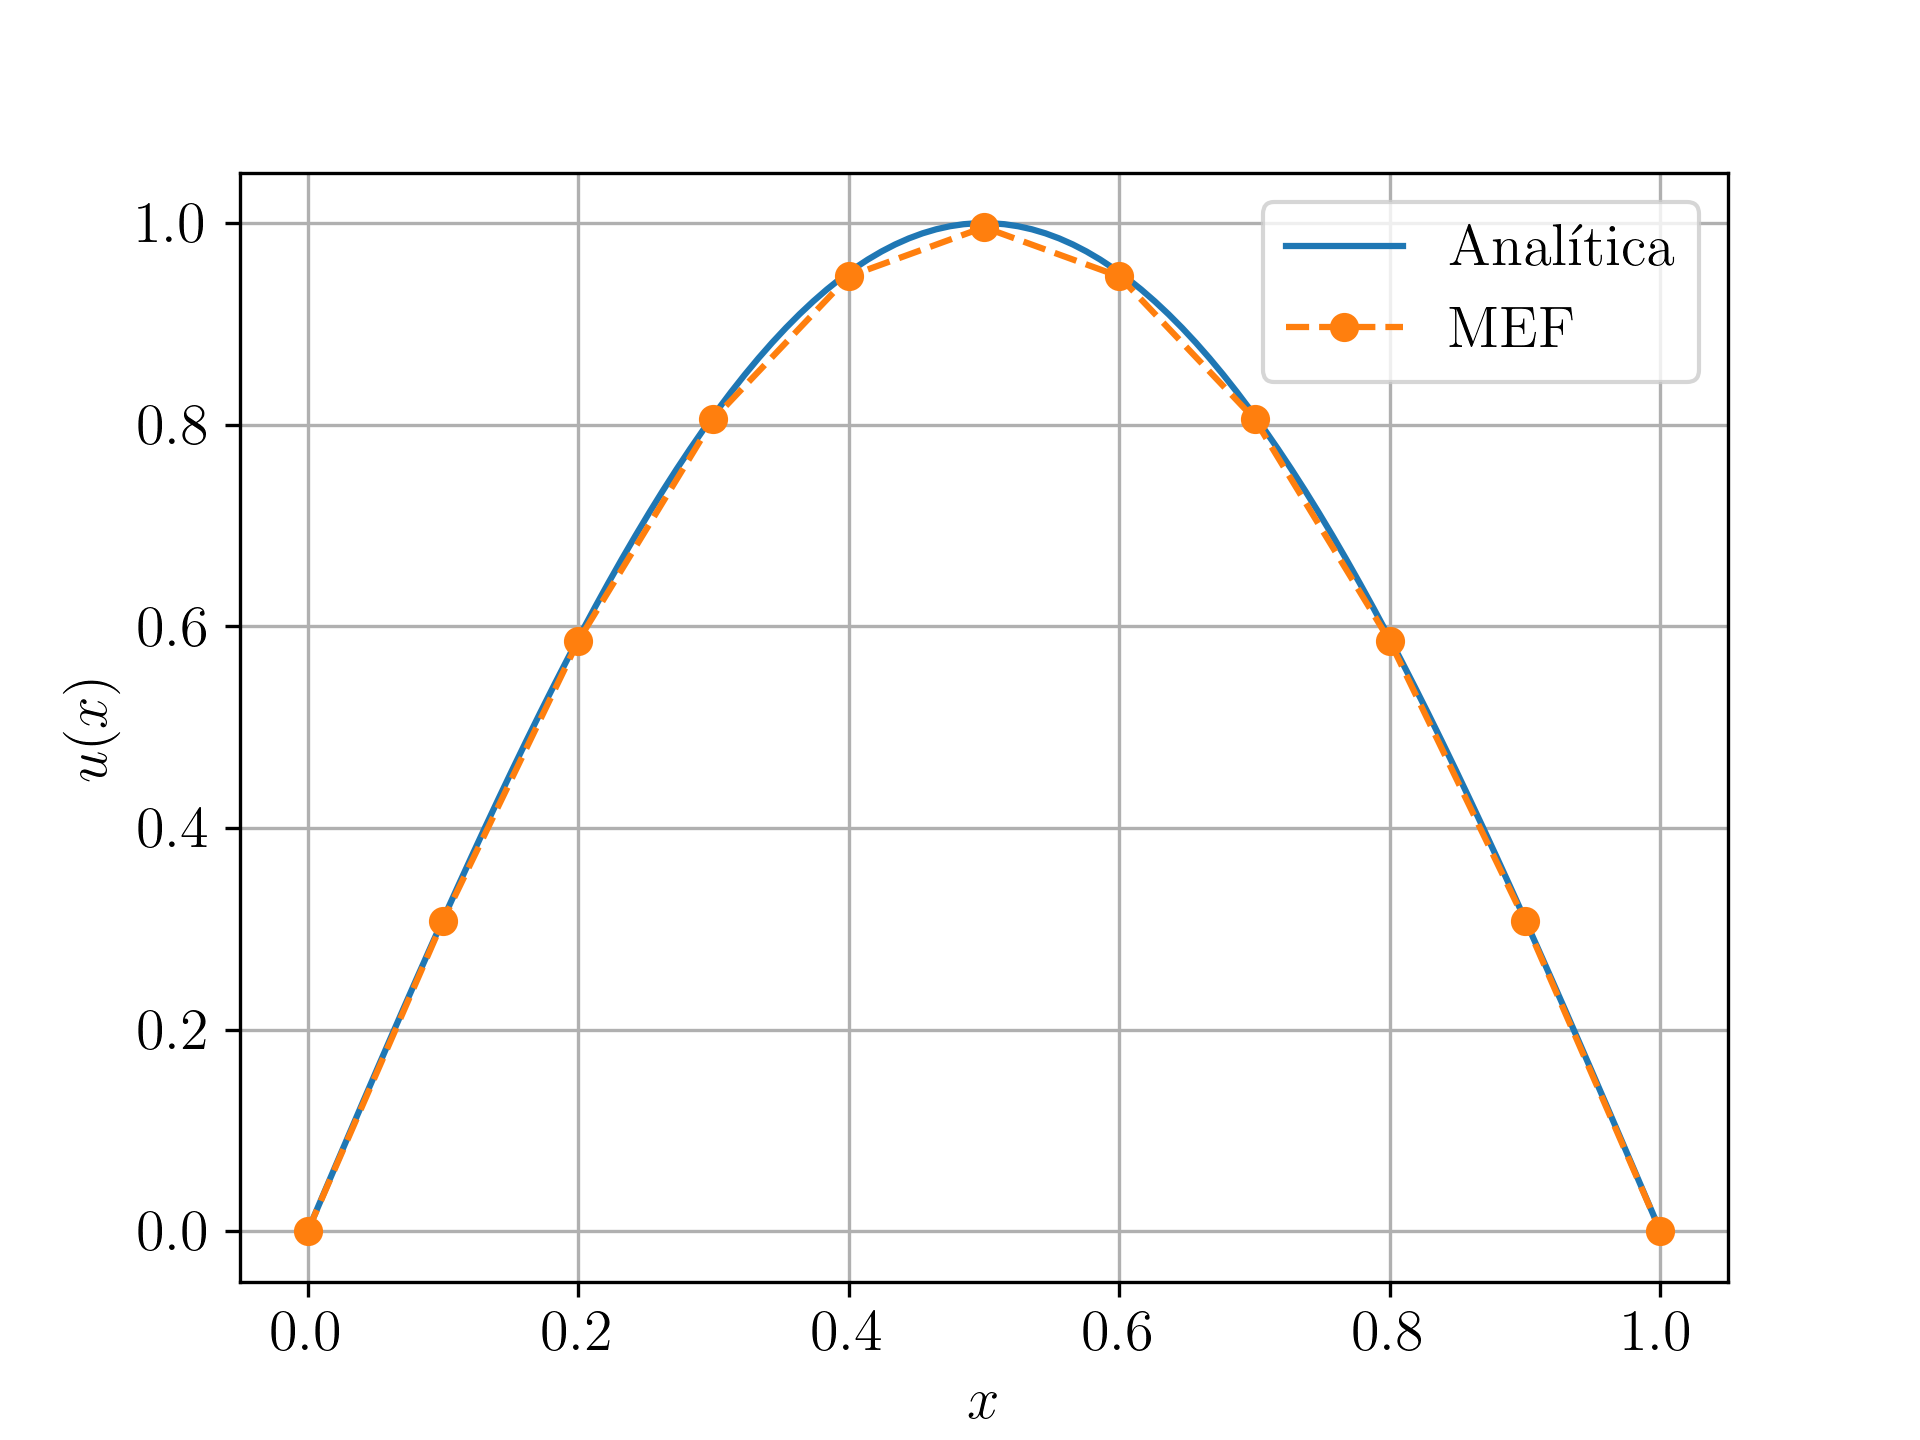
\includegraphics[width=0.8\textwidth]{./cap_pvc/dados/fig_mef/fig}
    \caption{Resultado referente ao Exemplo~\ref{cap_pvc_sec_mef:ex:pvc_mef}.}
    \label{cap_pvc_sec_mef:fig:ex_pvc_mef}
  \end{figure}

Resolvendo este sistema com $h=10^{-1}$ obtemos a solução numérica apresentada na Figura~\ref{cap_pvc_sec_mef:fig:ex_pvc_mef}.

\begin{lstlisting}[caption=pvc\_mef.py]
import numpy as np

# malha
n = 10
h = 1./n
xx = np.linspace(0., 1., n+1)

# fonte
def f(x):
    return np.pi**2*np.sin(np.pi*x)

# prob discreto
A = np.zeros((n-1, n-1))
b = np.empty(n-1)

# c.c. x = 0.
A[0,0] = 2./h
A[0,1] = -1./h
b[0] = h/2 * (f(xx[1]-0.5*h) + f(xx[1]+0.5*h))

# pts internos
for i in range(1,n-2):
    A[i,i-1] = -1./h
    A[i,i] = 2./h
    A[i,i+1] = -1./h
    b[i] = h/2 * (f(xx[i+1]-0.5*h) + f(xx[i+1]+0.5*h))

# c.c. x = 1.
A[n-2,n-3] = -1./h
A[n-2,n-2] = 2./h
b[n-2] = h/2 * (f(xx[n-1]-0.5*h) + f(xx[n-1]+0.5*h))

# resol
u = npla.solve(A, b)
## c.c. (dirichlet)
u = np.concatenate(([0.],u,[0.]))
\end{lstlisting}
\end{ex}

\subsection{Exercícios}

\begin{exer}
  Considere o PVC
  \begin{align}
    &-u'' = \pi^2\cos(\pi x), ~0 < x < 1,\\
    &u(0) = 1,\\
    &u(1) = -1.
  \end{align}
  A solução analítica deste problema é $u(x) = \cos(\pi x)$. Use o MEF para computar aproximações numéricas $\tilde{\pmb{u}}_h$ com tamanhos de malha $h=10^{-1}, 10^{-2}, 10^{-3}, 10^{-4}$ e verifique o erro absoluto $\varepsilon_{\text{abs}} := \|\tilde{\pmb{u}}_h - \pmb{u}\|$.
\end{exer}

\begin{exer}
  Considere o PVC
  \begin{align}
    &-u'' = 1, ~-1 < x < 1,\\
    &u(-1) = 0,\\
    &u(1) = 0.
  \end{align}
  A solução analítica deste problema é $u(x) = 1-x^2$. Use o MEF com $n=20$ subintervalos na malha e verifique o erro absoluto $\varepsilon_{\text{abs}} := \|\tilde{\pmb{u}}_h - \pmb{u}\|$. Por que o erro está próximo precisão de máquina? Justifique sua resposta.
\end{exer}

\begin{exer}
Considere o seguinte PVC
\begin{subequations}
  \begin{align}
    &-u'' + u' = f(x), ~-1 < x < 1,\\
    &u(-1) = 0,\\
    &u'(1) =0,
  \end{align}
\end{subequations}
onde
\begin{equation}
  f(x) = \left\{
    \begin{array}{ll}
      1 &, x\leq 0\\
      0 &, x>0
    \end{array}
  \right.
\end{equation}
Use uma aproximação adequada pelo MEF para obter o valor aproximado de $u(0)$ com precisão de $2$ dígitos significativos.
\end{exer}
\begin{resp}
  $7,2\E-1$
\end{resp}

\begin{exer}
  Considere o PVC
  \begin{align}
    &-u'' = \pi^2\cos(\pi x), ~0 < x < 1,\\
    &u(0) = 1,\\
    &u'(1) = 0.
  \end{align}
  A solução analítica deste problema é $u(x) = \cos(\pi x)$. Aplique o MEF para computar uma aproximação numérica com erro absoluto de no máximo $10^{-3}$ na norma $L^2$.
\end{exer}

\section{Método de Volumes Finitos}\label{cap_pvc_sec_mvf}

\hl{O \emph{Método de Volumes Finitos} (MVF) é um método de discretização apropriado para problemas conservativos}. Consideramos o seguinte problema linear de valor de contorno (PVC)
\begin{subequations}\label{cap_pvc_sec_mvf:eq:pvc}\hleq
  \begin{align}
    &-u_{xx} = f(x), ~a < x < b, \label{cap_pvc_sec_mvf:eq:pvc_eq}\\
    &u(a) = 0, \label{cap_pvc_sec_mvf:eq:pvc_bc1}\\
    &u(b) = 0. \label{cap_pvc_sec_mvf:eq:pvc_bc2}
  \end{align}
\end{subequations}
onde a incógnita é $u = u(x)$ com dada fonte $f = f(x)$. A Eq.~\eqref{cap_pvc_sec_mvf:eq:pvc} pode ser reescrita na forma conservativa
\begin{equation}
  \div(\pmb{F}) = f,
\end{equation}
onde $\pmb{F} = -u_x$

\begin{flushleft}
  \hlemph{1. Discretização Espacial.}
\end{flushleft}

Assumimos uma malha do domínio $[a, b]$ da forma
\begin{equation}
  a = x_{\frac{1}{2}} < x_1 < x_{\frac{3}{2}} < \cdots < x_{i-\frac{1}{2}} < x_i < x_{i+\frac{1}{2}} < \cdots < x_{n} < x_{n+\frac{1}{2}} = b,
\end{equation}
onde $h = (b-a)/n$, $x_{i-\frac{1}{2}} = a + (i-1)h$, $h^{-} = h^{+} = h/2$, $i = 1, 2, \dotsc, n$. Também denotamos $K_i = \left(x_{i-\frac{1}{2}}, x_{i+\frac{1}{2}}\right)$ a $i$-ésima célula da malha.

\begin{flushleft}
  \hlemph{2. Discretização das Equações.}
\end{flushleft}

No MVF, as incógnitas $u_i$, $i = 1, 2, \dotsc, n$, são as aproximações para o valor médio de $u$ nas células $K_i$, i.e.
\begin{equation}
  u_i = \frac{1}{|K_i|}\int_{a}^{b}u(x)\,dx.
\end{equation}
O sistema discreto para $u_i$ é obtido tomando a média da Eq.~\label{cap_pvc_sec_fem:eq:pvc_eq} na célula $K_i$, donde temos
\begin{subequations}
  \begin{align}
    &-\frac{1}{h}\int_{x_{i-\frac{1}{2}}}^{x_{i+\frac{1}{2}}}u_{xx}\,dx = \frac{1}{h}\int_{K_i}f\,dx,\\
    &\hleq \frac{1}{h}\left[-u_x\left(x_{i+\frac{1}{2}}\right) + u_x\left(x_{i-\frac{1}{2}}\right)\right] = \frac{1}{h}\int_{K_i}f\,dx\label{cap_pvc_sec_mvf:eq:aux00}
  \end{align}
\end{subequations}
Por fórmula de diferenças finitas central, temos
\begin{equation}
  u_{x}\left(x_{i+\frac{1}{2}}\right) = \frac{u_i - u_{i-1}}{h} + O(h)
\end{equation}
e
\begin{equation}
  u_x\left(x_{i-\frac{1}{2}}\right) = \frac{u_{i+1} - u_i}{h} + O(h)
\end{equation}
Com isso, obtemos as equações
\begin{equation}\label{cap_pvc_sec_mvf:eq:aux0}
  \frac{1}{h}\left(-\frac{u_{i+1}-u_{i}}{h} + \frac{u_i - u_{i-1}}{h}\right) = \frac{1}{h}\int_{K_i}f\,dx,
\end{equation}
Rearranjando os termos e aproximando a integral de $f$ pela \href{https://notaspedrok.com.br/notas/MatematicaNumericaII/cap_integr_sec_nc.html}{\emph{regra do ponto médio}}, obtemos
\begin{equation}\label{cap_pvc_sec_mvf:eq:aux}
  -\frac{1}{h^2}u_{i-1} + \frac{2}{h^2}u_i - \frac{1}{h^2}u_{i+1} = f_i,
\end{equation}
onde $f_i := f(x_i)$ e $i = 2, 3, \dotsc, n-1$.

Na célula $K_1$, tomamos a aproximação
\begin{subequations}
  \begin{align}
    u_x\left(x_{\frac{1}{2}}\right) &= \frac{u_{1} - u_{\frac{1}{2}}}{h/2} + O\left(h\right),\\
                                    &= = \frac{u_{1}}{h/2} + O\left(h\right).
  \end{align}
\end{subequations}
Aplicando na Eq.~\eqref{cap_pvc_sec_mvf:eq:aux00}, obtemos
\begin{equation}\hleq
  \frac{1}{h}\left(-\frac{u_{2}-u_{1}}{h} + \frac{u_1}{h/2}\right) = \frac{1}{h}\int_{K_i}f\,dx,
\end{equation}
Analogamente, integrando na célula $K_n$ de fronteira, obtemos
\begin{equation}\hleq
  \frac{1}{h}\left(\frac{u_{n}}{h/2} + \frac{u_{n} - u_{n-1}}{h}\right) = \frac{1}{h}\int_{K_i}f\,dx.
\end{equation}

Por fim, obtemos o \hlemph{sistema discreto}
\begin{subequations}\hleq
  \begin{align}
    &\frac{3}{h^2}u_1 - \frac{1}{h^2}u_{2} = f_1,\\
    &-\frac{1}{h^2}u_{i-1} + \frac{2}{h^2}u_i - \frac{1}{h^2}u_{i+1} = f_i,\\
    &-\frac{1}{h^2}u_{n-1} + \frac{3}{h^2}u_{n+1} = f_n,
  \end{align}
\end{subequations}
para $i = 2, 3, \dotsc, n-1$.

\begin{ex}\label{cap_pvc_sec_mvf:ex:pvc_mvf}
  Consideramos o seguinte PVC
  \begin{align}
    &-u'' = \pi^2\sen(\pi x), ~0 < x < 1,\\
    &u(0) = 0,\\
    &u(1) = 0.
  \end{align}
  A solução analítica deste problema é $u(x) = \sen(\pi x)$.
  
  \begin{figure}[h!]
    \centering
    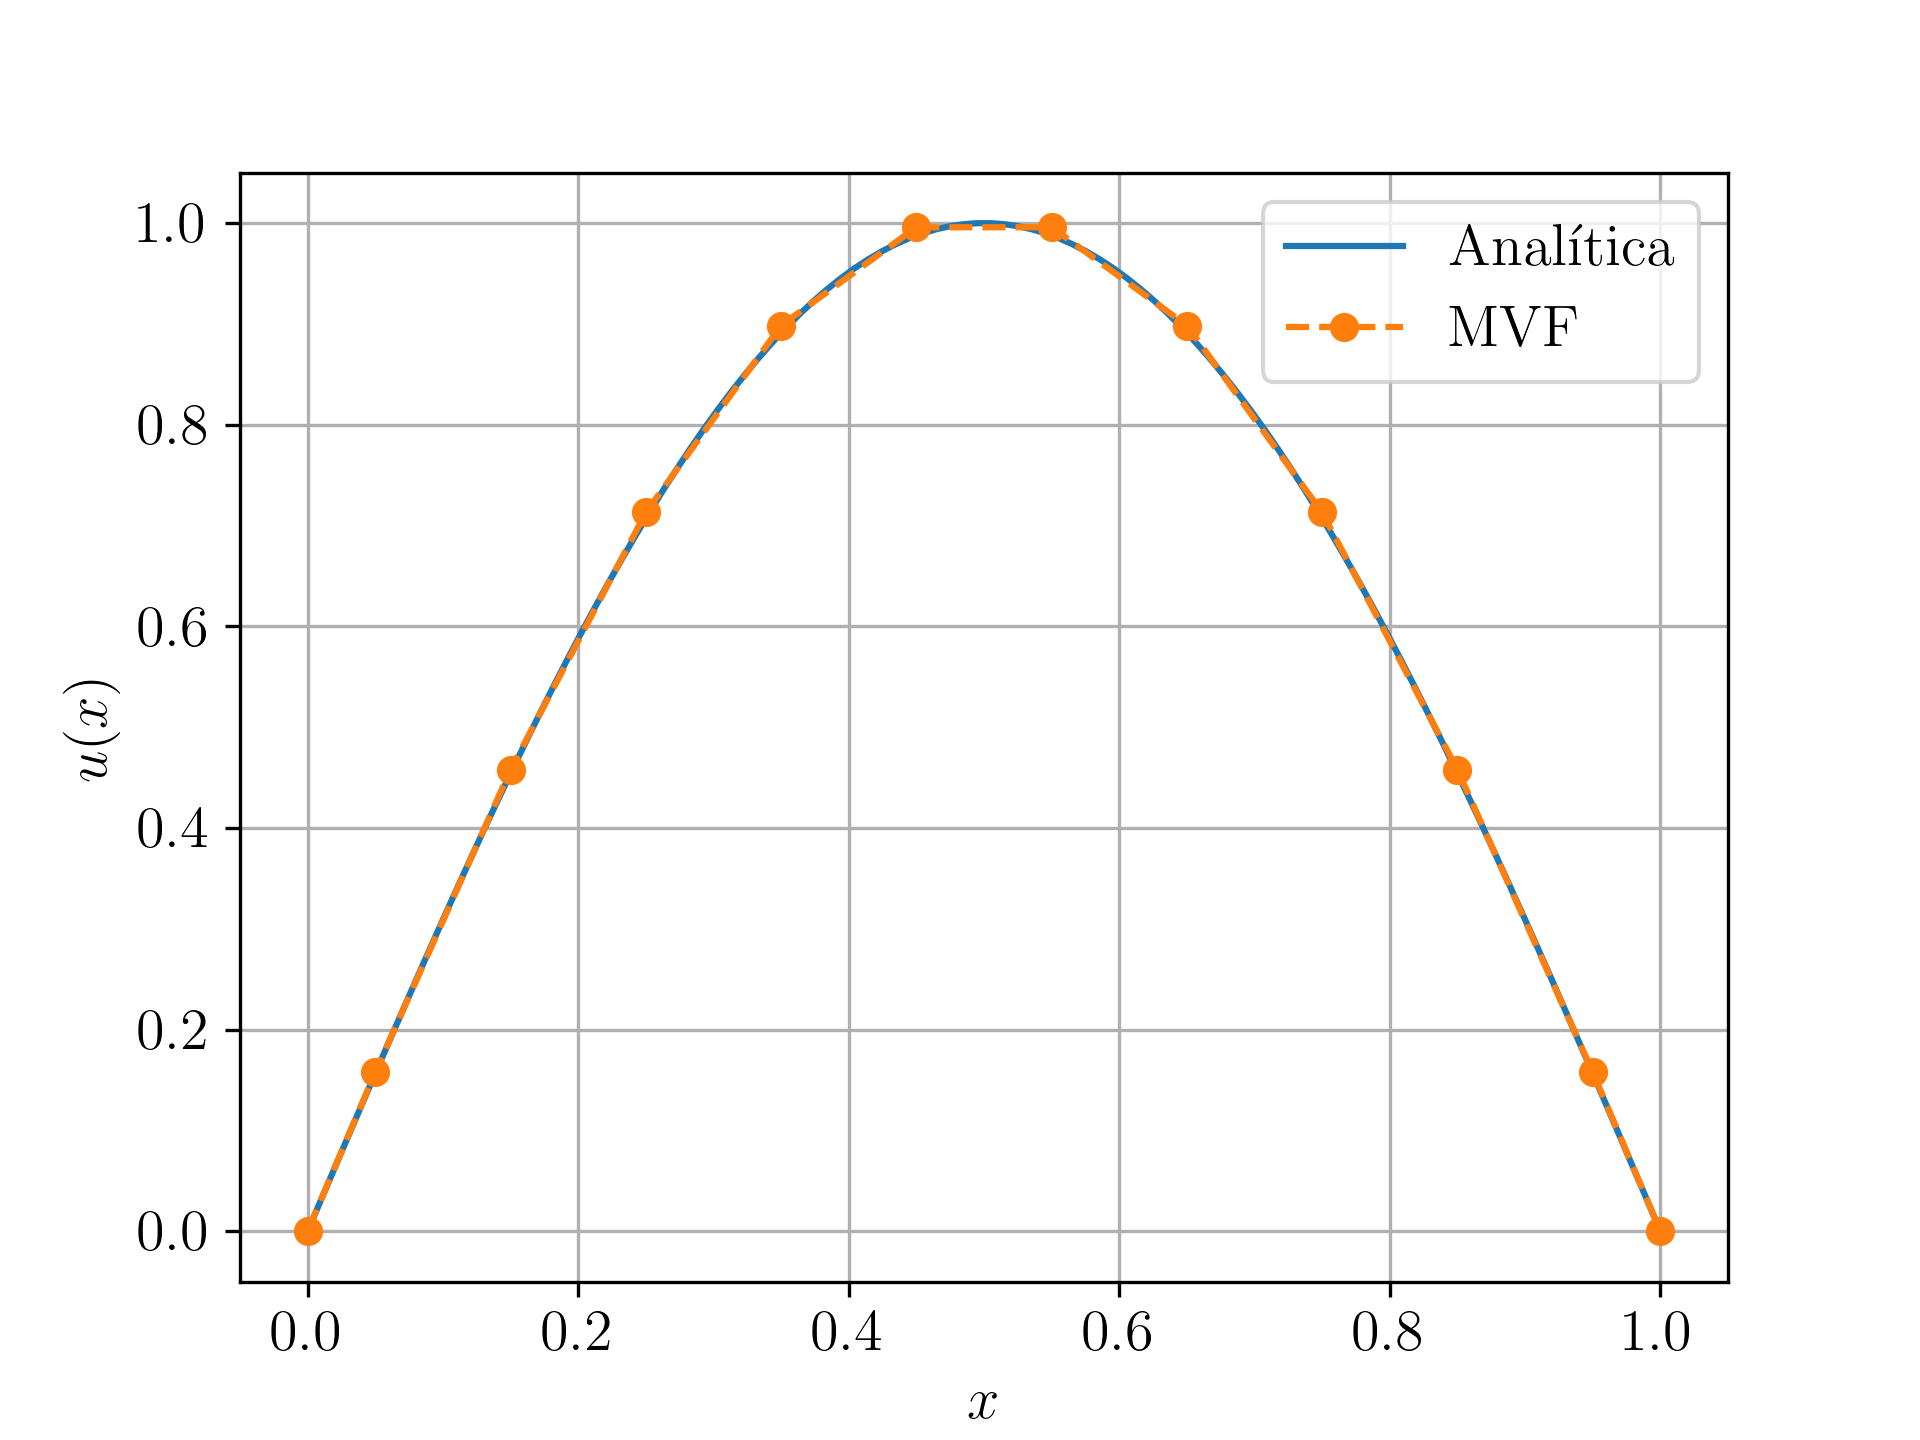
\includegraphics[width=0.8\textwidth]{./cap_pvc/dados/fig_mvf/fig}
    \caption{Resultado referente ao Exemplo~\ref{cap_pvc_sec_mef:ex:pvc_mvf}.}
    \label{cap_pvc_sec_mvf:fig:ex_pvc_mvf}
  \end{figure}

  Resolvendo este sistema com $h=10^{-1}$ obtemos a solução numérica apresentada na Figura~\ref{cap_pvc_sec_mvf:fig:ex_pvc_mvf}.

\begin{lstlisting}[caption=pvc\_mvf.py]
import numpy as np

# fonte
def f(x):
  return np.pi**2*np.sin(np.pi*x)

# malha
n = 10
h = 1./n
xx = np.linspace(h/2, 1.-h/2, n)

# prob. discreto
A = np.zeros((n,n))
b = np.empty(n)

# c.c. x = 0
A[0,0] = 3./h**2
A[0,1] = -1./h**2
b[0] = f(xx[0])

# pts internos
for i in range(1,n-1):
  A[i,i-1] = -1./h**2
  A[i,i] = 2./h**2
  A[i,i+1] = -1./h**2
  b[i] = f(xx[i])

# c.c. x = 1
A[n-1,n-2] = -1./h**2
A[n-1,n-1] = 3./h**2
b[n-1] = f(xx[n-1])

# resol prob disc
u = npla.solve(A, b)

xx = np.concatenate(([0.],xx,[1.]))
u = np.concatenate(([0.],u,[0.]))
\end{lstlisting}
\end{ex}

\subsection{Exercícios}

\begin{exer}
  Considere o PVC
  \begin{align}
    &-u'' = \pi^2\cos(\pi x), ~0 < x < 1,\\
    &u(0) = 1,\\
    &u(1) = -1.
  \end{align}
  A solução analítica deste problema é $u(x) = \cos(\pi x)$. Use o MVF para computar aproximações numéricas $\tilde{\pmb{u}}_h$ com tamanhos de malha $h=10^{-1}, 10^{-2}, 10^{-3}, 10^{-4}$ e verifique o erro absoluto $\varepsilon_{\text{abs}} := \|\tilde{\pmb{u}}_h - \pmb{u}\|$.
\end{exer}

\begin{exer}
  Considere o PVC
  \begin{align}
    &-u'' = 1, ~-1 < x < 1,\\
    &u(-1) = 0,\\
    &u(1) = 0.
  \end{align}
  A solução analítica deste problema é $u(x) = 1-x^2$. Use o MVF com $n=20$ subintervalos na malha e verifique o erro absoluto $\varepsilon_{\text{abs}} := \|\tilde{\pmb{u}}_h - \pmb{u}\|$.
\end{exer}

\begin{exer}
Considere o seguinte PVC
\begin{subequations}
  \begin{align}
    &-u'' + u' = f(x), ~-1 < x < 1,\\
    &u(-1) = 0,\\
    &u'(1) =0,
  \end{align}
\end{subequations}
onde
\begin{equation}
  f(x) = \left\{
    \begin{array}{ll}
      1 &, x\leq 0\\
      0 &, x>0
    \end{array}
  \right.
\end{equation}
Use uma aproximação adequada pelo MVF para obter o valor aproximado de $u(0)$ com precisão de $2$ dígitos significativos.
\end{exer}
\begin{resp}
  $7,2\E-1$
\end{resp}

\begin{exer}
  Considere o PVC
  \begin{align}
    &-u'' = \pi^2\cos(\pi x), ~0 < x < 1,\\
    &u(0) = 1,\\
    &u'(1) = 0.
  \end{align}
  A solução analítica deste problema é $u(x) = \cos(\pi x)$. Aplique o MVF para computar uma aproximação numérica com erro absoluto de no máximo $10^{-3}$ na norma $L^2$.
\end{exer}
